%\section{Introduction}

\subsection{Motivation}
\label{chapter:motivation}

With every consecutive year, the information processing technologies advance in functionality and performance, leading to improvements in information capture, transmission, storage, and subsequent manipulations. 

In modern imaging devices, one of the most significant performance metrics is the spatial resolution of the system, expressed as the amount of resolvable information per unit of space. High resolution is crucial for distinguishing structures located within a small proximity to each other. Resolution improves with the shrinkage of the imaging elements, e.g. pixels in a sensor, and allows for more precise representations while potentially retaining the same system size in general. 

Such developments are generally desired: while not necessarily as significant for the most conventional consumer imaging devices, improved accuracy and reconstruction of the data is pivotal for a number of domains. These include remote sensing for astronomical imaging, microscopy research in biological sciences, prognostics, and medical examinations, and many more. Super-resolution is equally important in industrial applications, where the amount of data available for intepretation can be used in computer vision tasks such as object recognition or traffic surveillance.%, general prognostics, and medical examinations.
\cite{SResolution, Anwar2020ADJ}  

\subsection{State of the Art}
The current implementations tend to make use of the established digital sensor technology standard, the CMOS active pixel imaging sensor with intra-pixel charge transfer. Often described as a "camera-on-a-chip" technology, the conventional CMOS image sensor (CIS for short) has found use in both consumer and industrial applications due to its low-power consumption, high level of integration and small manufacturing sizes~\cite{8454568}. 

The highest resolution pixel-wise in current imaging devices is nearing 150 MP~\cite{lawton_artaius_2021}, where it's partially associated with larger sensor formats, sacrificing the compact size in the process for insignificantly larger amount of picture elements. High prices render such cameras unattainable for an average consumer. Besides the actual acquisition process, existing images have to be reconstructed in higher resolutions as well.

\subsubsection{Software-Based Implementations}

Many existing image processing approaches can be employed to enhance spatial resolution in existing \textit{low resolution} (LR) images. Based entirely in the software domain, such solutions require nothing but computational power and are utilized the most, to the point of being synonymous with the term ``gigapixel imaging'' itself.

The image recreation process is data-driven: the input can be a single image, or consist of a dataset of similar images with insubstantial differences from one another. Similarly, the methods employed can be based on the computer vision algorithms in the traditional sense or involve deep learning network architectures, which require an additional source of data in order to be outperforming the prior~\cite{Anwar2020ADJ}.

\paragraph{Image Stitching}

Image stitching techniques explicitly require abundant, spatially and temporally coherent image datasets with overlapping regions. The most common application of such techniques consists in the production of high-resolution panoramic images, which can then be   utilized for entertainment or preservation purposes~\cite{7136690}.

By now, the production of the panoramic gigapixel images is steadily made available to the consumers. A fine example is the GigaPan technology~\cite{GigaPanWWW}, which stems from the collaboration between Carnegie Mellon University, NASA Robotics Group, and Google; since then, it has been spun off into a commercial service offering both hardware accommodations and the software, thus defining a clear, streamlined workflow. The solutions encompass a designated robotic mount facilitating continuous image capture through panning along its axis, a corresponding image stacking software, and even a web-based interface for sharing the composite image afterwards. 

The camera mount is meant for use with any amateur DSLR camera, meaning that the exact resolution of the resulting panorama is dependent on the dimensions of the optical components and the sensor model. The demonstration of the process can be found online \cite{GigaPanVimeo}.

\paragraph{Image Synthesis via Deep Learning}

Deep learning-

based methods are best employed for a reconstruction of a single low-resolution image. 

The super-resolution version of a single image is by definition an under-determined problem with a multitude of possible solutions. Classical computer vision algorithms don't fare well in such tasks, as the recovery of such images may lead to the propagation of wrong information. For an accurate reproduction of the scene, one may need reliable prior information which relates to the human perception in a meaningful way. 

The objects depicted in the image can be upsampled based on their predicted taxonomy and feature sets, which is one of the main applications of the convolutional neural networks. Depending on the data involved in the training, the interpolated data could be refined in many ways; for instance, distinguished objects could have their corresponding surfaces refined based on their class, filling in the structures with already available high-resolution textures of the corresponding materials.

A number of network designs, varying widely in their complexity, depth, training data, and features, has been considered for the gigapixel imaging. An extensive overview on the available architectures can be found in \cite{Anwar2020ADJ} and \cite{10.1007/978-3-030-36808-1_37}.
 
 
\paragraph{Applicability}

One should note that neither image stitching nor image synthesis techniques are exclusive to the gigapixel imaging in their methodology; working with a sequence of images in particular is a challenge which quickly turns into an image registration problem, requiring integrated solutions regarding tonemapping, uneven illumination, projective distortions of the depicted objects etc. For this reason alone, the strictly software-based solutions pose no special challenge to the gigapixel imaging and are therefore declared out of scope of this paper.

\subsubsection{Hardware-Based Implementations} 

The computational complexity of the problem can be reduced by addressing it on a lower level of abstraction. Here, the focus lies on acquiring the super-resolution directly by means of the appropriate hardware architecture design. With this, the need for elaborate LR datasets lapses as well. 

Several solutions focusing on the predominantly hardware-based domain exist. %underlying analog circuit components
 
\paragraph{Scanning}

A popular imaging solution involves a flatbed scanner capable of relatively high scanning resolution (commonly provided in dots per inch, or DPI): with most consumer scanning devices supporting 300 dpi and above, this off-chip solution is both low-cost and widely available. 
 \begin{figure}[h]
  \centering
  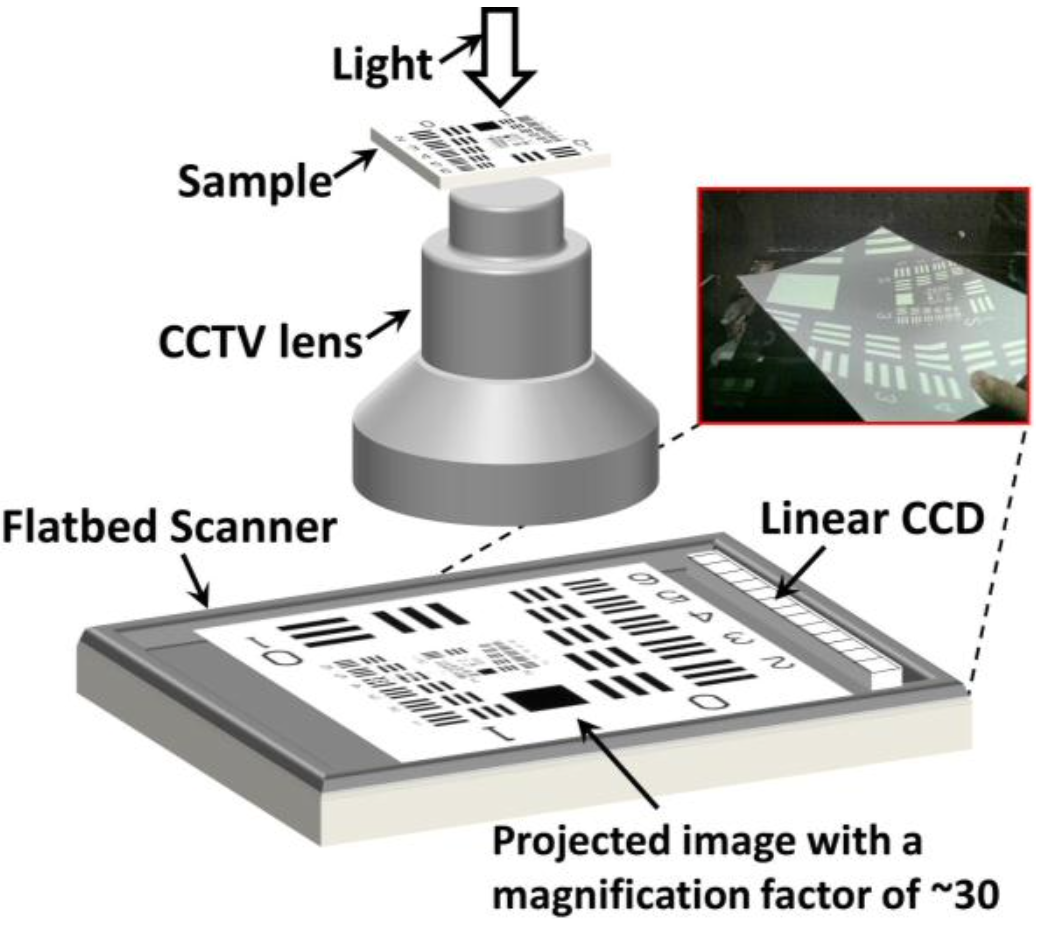
\includegraphics[width=0.7\linewidth]{imgs/gigascan.png}
  \caption{The proof-of-concept gigapixel microscopy setup, as demonstrated in \cite{zheng20140}. The scanner at hand can resolve 2400dpi, which corresponds to the pixel size of ca. 10$\mu$m.}
  \label{fig:gigamicro}
  \Description{Proposal for a gigapixel imaging setup for usage in microscopy. Depicted are generic flatbed scanner, a lens, and a sample to be captured. The sample is illuminated and positioned next to the optical system such that a magnified image appears, projected onto the scanning area.}
\end{figure}

In gigapixel solutions tailored specifically to microscopy research, the scanners register magnified projections of the input samples \cite{Zheng:12};
% previously magnified via a  closed-circuit-television lens
other papers attempt to enhance the scanning process by modifying the scanner device directly \cite{ConfocalScan}, or using alternative scanning methods (e.g. tilt scanning in \cite{tileScan}).

 %\begin{figure}[h]
%  \centering
%  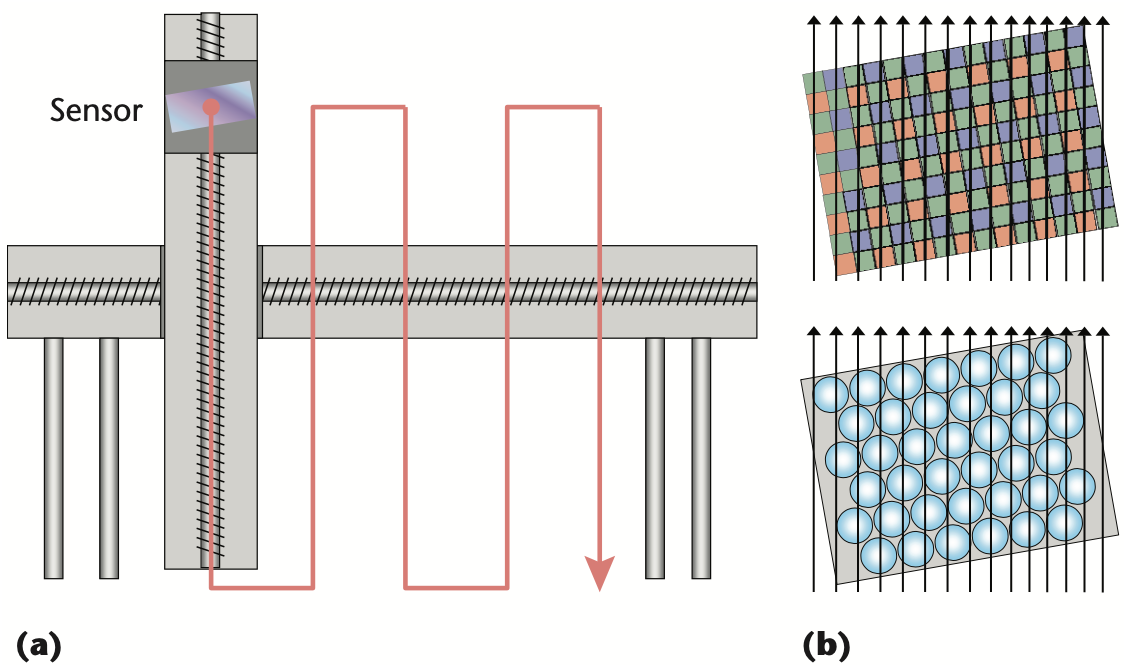
\includegraphics[width=\linewidth]{imgs/scantech.png}
%  \caption{Tilt scanning techniques presented in \cite{tileScan}.}
%  \Description{Scanning can be performed diagonally, where the new direction doesn't fit the singular pixels exactly, and each detector fits somewhere in the middle. Through such incoherences, one can oversample the light field similar to the phase shift method.}
%\end{figure}

%Projection-based scan methods may contain redundancies depending on the source. For instance, light intereference should be taken into account; with analog media, one risks introducing further factors into the equation, as the optical density in a print image will also depend on the properties of the photographic medium (paper, ink, etc.), the device used for printing, and present physical foreign particles, such as dust. In this case, the quantity does not necessarily substitute the quality, and the higher spatial resolution merely leads to the redundancies in data, thus not influencing the information content itself in any way.

\paragraph{Composite of Sensor Arrays}
An attempt to attain high resolution in the digital domain using existing technologies is a popular method in large scale applications. 

Widely used in airborne and astronomical systems are precision-mosaicked sensor arrays. In this case, conventional MP-sized imaging sensors are brought together into an array and treated as a whole. Since the optical components of the system are mostly unchanged, this is a fixed-focus system. %; similarly, the same step can be applied to preceding optical components of the system. 

Such cascading architectures are rather unwieldly, expensive, and is therefore mostly found in research facilities, where the rigidity of the architecture is unimportant. This stacked sensor technology can be seen in airborne and astronomical systems such as ARGUS, LSST and Pan-STARR~\cite{multiscale}.

Alternatively, the system can employ multicameras, allowing for a multi-scaled approach. One of such gigapixel camera architectures is AWARE, developed by The Duke Information Spaces Project. AWARE employs arrays of microcameras, using a monocentric lens objective as the primary optical component. The first generation, AWARE-2, consisted of 98 microcameras on a monochromatic CMOS sensor, producing a 1.0 gigapixel image spanning a 120$\deg$ × 40$\deg$ field of view~\cite{GongGPU}. Since then, a variety of models have been developed, enabling color acquisition and ranging in optical resolution, size, and amount of microcameras. There are operational advantages to AWARE as well, since each camera can be independently controlled in acquisition settings~\cite{multiscale}. Summarized, such multilens cameras are more compact and serve well in terrestrial applications. \cite{aware2}

 \begin{figure}[h]
  \centering
  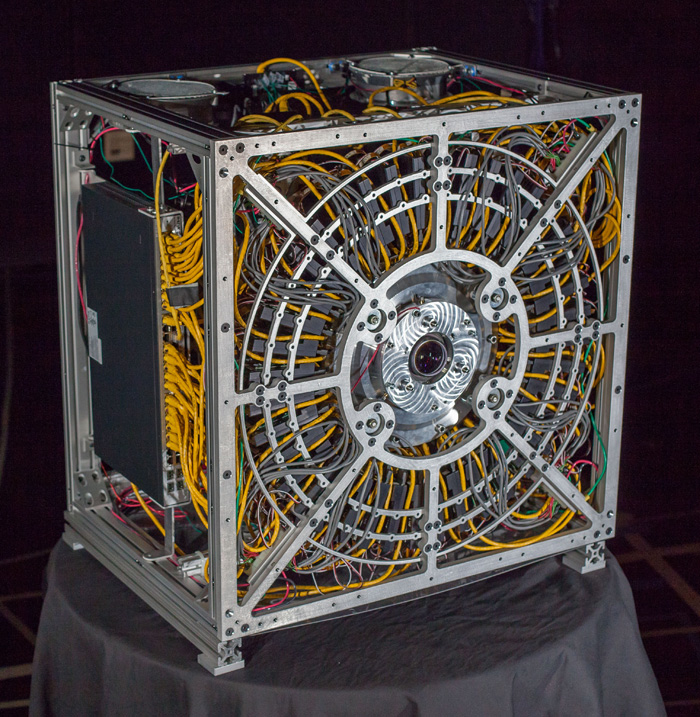
\includegraphics[width=0.5\linewidth]{imgs/aware.jpg}
  \caption{AWARE-2 camera design, via: \cite{physics_world_2018}}
  \Description{AWARE-2, one of the multilens camera designs presented in the paper}
\end{figure}

\paragraph{Photon-Counting}
The latest advancements in the manufacturing of integrated circuits (ICs) have put us in the post-Moore's law era. 

From 1970s on \cite{Cerofolini2007}, the complexity of the circuitry would grow at a much higher rate than once theorized, while the physical dimensions of the semiconductors would scale down. By 2020, the possible pixel pitch in CMOS sensors can be as low as 3$n$m~\cite{hao2021recent}, meaning that the sensor dimensions used in current photographic devices can now hold significantly larger pixel amounts, providing us with higher spatial resolution in an image. However, at the present time the pixel dimensions are approaching physical limits: by reducing the pixel area, the full-well [photoelectron charge] capacity of a singular pixel, too, is lowered. This has grave implications for the image quality, as the small difference between the signal and the noise decreases the dynamic range. 

The solution to overcoming the trend of pixel shrinkage while maintaining the higher resolution has been proposed by Eric R. Fossum in 2005.%, an inventor of CMOS. 

Sufficiently small pixels should only be able to store charge of one photoelectron alone.  Each of those pixels can then assume values of either 0, meaning no photons have reached the light-sensitive sensor plane, or 1, signifying that at least one has struck the surface after all, resulting in registered exposure. The sensor response lies in a binary range. The actual evaluation of the sensor data, i.e. the image formation, happens post-capture via analysis of the Poisson distribution of the photons over multiple observations in time, and can be managed dynamically. 

Photon-counting, or, quantum imaging sensors can ultimately represent a paradigm shift in photography. Since its introduction, the binary sensor has been applied and conceptualized in many ways.% Such devices will be the main focus of this report. 
